\documentclass[a4paper, 14pt]{extarticle}

\usepackage{../generalPreamble}
\usepackage{../reportFormat}


\begin{document}

\begin{titlepage}
    \centering
    {\bfseries
        \uppercase{
            Минобрнауки России \\
            Санкт-Петербургский государственный \\
            Электротехнический университет \\
            \enquote{ЛЭТИ} им. В.И.Ульянова (Ленина)\\
        }
        Кафедра ИБ

        \vspace{\fill}
        \uppercase{Лабораторная работа №3} \\
        по дисциплине \enquote{Криптография и защита информации} \\
        Тема: Изучение классических шифров Hill, ADFGVX, Playfair
    }

    \vspace{\fill}
    \begin{tabularx}{0.8\textwidth}{l X c r}
        Студент гр. 6304 & & \underline{\hspace{3cm}} & Корытов П.В.\\
        Преподаватель & & \underline{\hspace{3cm}} & Племянников А.К.
    \end{tabularx}

    \vspace{1cm}
    Санкт-Петербург \\
    \the\year{}
\end{titlepage}

\newpage

\section*{Цель работы}
Цель работы: исследовать шифры Hill, ADFGVX, Playfair и получить практические навыки работы с ними, в том числе и в программном продукте CrypTool 1 и 2.

\section{Шифр Хилла}
\subsection{Описание шифра}
Зашифровка шифром Хилла:

\begin{table}[h]
    \centering
    \begin{tabular}{@{}lllllllllllll@{}}
    \toprule
    \textbf{A} & \textbf{B} & \textbf{C} & \textbf{D} & \textbf{E} & \textbf{F} & \textbf{G} & \textbf{H} & \textbf{I} & \textbf{J} & \textbf{K} & \textbf{L} & \textbf{M} \\
    \textit{0} & \textit{1} & \textit{2} & \textit{3} & \textit{4} & \textit{5} & \textit{6} & \textit{7} & \textit{8} & \textit{9} & \textit{10} & \textit{11} & \textit{12} \\ \midrule
    \textbf{N} & \textbf{O} & \textbf{P} & \textbf{Q} & \textbf{R} & \textbf{S} & \textbf{T} & \textbf{U} & \textbf{V} & \textbf{W} & \textbf{X} & \textbf{Y} & \textbf{Z} \\
    \textit{13} & \textit{14} & \textit{15} & \textit{16} & \textit{17} & \textit{18} & \textit{19} & \textit{20} & \textit{21} & \textit{22} & \textit{23} & \textit{24} & \textit{25} \\ \bottomrule
    \end{tabular}
\end{table}
Текст --- \texttt{HILLCIPHEREXAMPLES}

\begin{equation*}
    \left(\begin{matrix}
        7 & 8 & 11 \\
        11 & 2 & 8 \\
        15 & 7 & 4\\
        17 & 4 & 23\\
        0 & 12 & 15\\
        11 & 4 & 18
    \end{matrix}\right) \times
    \underbracket[0pt][0pt]{%
    \left(\begin{matrix}
        6 & 24 & 1 \\
        13 & 16 & 10 \\
        20 & 17 & 15
    \end{matrix}\right)}_{\text{Шифрующая матрица}} = 
    \left( \begin{matrix}
        366 & 483 & 522\\
        252 & 432 & 151\\
        261 & 540 & 145\\
        614 & 863 & 402\\
        456 & 447 & 345\\
        478 & 634 & 321\\
    \end{matrix} \right) \equiv
    \left( \begin{matrix}
        2 & 15 & 18\\
        18 & 16 & 21\\
        1 & 20 & 15\\
        16 & 5 & 12\\
        14 & 5 & 7\\
        10 & 10 & 9
    \end{matrix} \right) (\bmod 26)
\end{equation*}

Шифротекст: \texttt{CPSSQVBUPQFMOFHKKJ}

Требования к шифрующей матрице --- она должна быть обратима, т.е. $|M| \ne 0$. В таком случае $M^{-1}$ --- мультипликативная инверсия в $\mathbb{Z}_{26}$: $M \times M^{-1} \equiv I \bmod 26 $

Расшифровка:
\begin{equation*}
    \left( \begin{matrix}
        2 & 15 & 18\\
        18 & 16 & 21\\
        1 & 20 & 15\\
        16 & 5 & 12\\
        14 & 5 & 7\\
        10 & 10 & 9
    \end{matrix} \right) \times
    \underbracket[0pt][0pt]{%
    \left( \begin{matrix}
        8 & 5 & 10\\
        21 & 8 & 21\\
        21 & 12 & 8
\end{matrix} \right)}_{\text{Обратная матрица}} = 
    \left( \begin{matrix}
        709 & 346 & 479\\
        921 & 470 & 684\\
        743 & 345 & 550\\
        485 & 264 & 361\\
        364 & 194 & 301\\
        479 & 238 & 382
    \end{matrix}\right) \equiv
    \left(\begin{matrix}
        7 & 8 & 11 \\
        11 & 2 & 8 \\
        15 & 7 & 4\\
        17 & 4 & 23\\
        0 & 12 & 15\\
        11 & 4 & 18
    \end{matrix}\right) (\bmod 26)
\end{equation*}
\subsection{Формулировка задания}
\begin{enumerate}
    \item Найти шифр в CrypTool 1: Encrypt/Decrypt-> Symmetric (Classic).
    \item Зашифровать и расшифровать текст содержащий только фамилию (транслитерация латиницей) вручную и с помощью шифра c выбранным ключом 2х2. Убедиться в совпадении результатов. Проверить обратимость шифрующей матрицы (ключа).
    \item Зашифровать текст с произвольным сообщением в формате `DEAR MR ФАМИЛИЯ ИМЯ ОТЧЕСТВО THANK YOU VERY MUCH'', используя транслитерацию латиницей и шифрующую матрицу 3х3.
    \item Выполнить атаку на основе знания открытого текста, используя приложение из Analysis-> Symmetric Encryption (classic)-> Known Plaintext.
    \item Удалить из сообщения и шифротекста фрагменты с ФАМИЛИЯ ИМЯ ОТЧЕСТВО и повторить атаку. Убедиться, что полученный ключ (матрица) совпадает с исходным.
    \item Передайте произвольную шифровку коллеге для расшифрования при условии, что формы обращения и завершения сообщения известны. Размер использованного ключа держать в секрете.
\end{enumerate}

\subsection{Ход работы}
\begin{enumerate}
    \item Найден шифр в CrypTool1. Параметры шифра на рисунке~\ref{img:1:1}
    \begin{figure}[h]
        \centering
        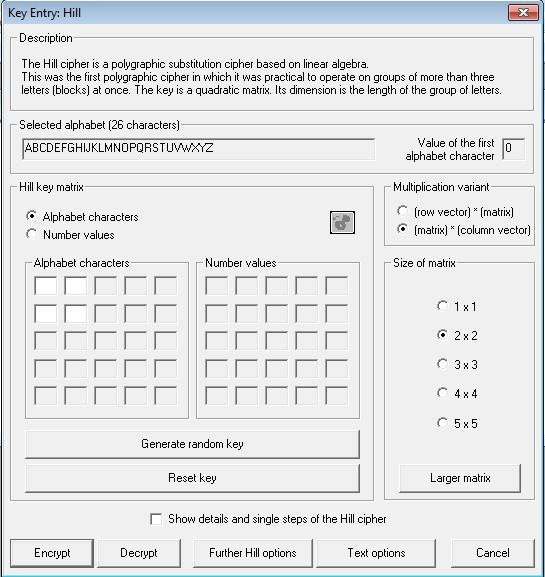
\includegraphics[width=0.7\textwidth]{./img/S003.jpg}
        \caption{Параметры шифра Хилла}%
        \label{img:1:1}
    \end{figure}
    \item Фамилия автора --- \texttt{KORYTOV}
    \begin{table}[h]
        \centering
        \begin{tabular}{@{}lllllllllllll@{}}
        \toprule
        \textbf{A} & \textbf{B} & \textbf{C} & \textbf{D} & \textbf{E} & \textbf{F} & \textbf{G} & \textbf{H} & \textbf{I} & \textbf{J} & \textbf{K} & \textbf{L} & \textbf{M} \\
        \textit{0} & \textit{1} & \textit{2} & \textit{3} & \textit{4} & \textit{5} & \textit{6} & \textit{7} & \textit{8} & \textit{9} & \textit{10} & \textit{11} & \textit{12} \\ \midrule
        \textbf{N} & \textbf{O} & \textbf{P} & \textbf{Q} & \textbf{R} & \textbf{S} & \textbf{T} & \textbf{U} & \textbf{V} & \textbf{W} & \textbf{X} & \textbf{Y} & \textbf{Z} \\
        \textit{13} & \textit{14} & \textit{15} & \textit{16} & \textit{17} & \textit{18} & \textit{19} & \textit{20} & \textit{21} & \textit{22} & \textit{23} & \textit{24} & \textit{25} \\ \bottomrule
        \end{tabular}
    \end{table}
    \begin{equation*}
        |A| = \left| \begin{matrix} 1 & 2 \\ 3 & 4 \end{matrix} \right| = 1 * 4 - 3 * 2 = -2
    \end{equation*}
    Матрица шифрования обратима

    \begin{equation*}
        \left( \begin{matrix}
            10 & 14 \\
            17 & 24 \\
            19 & 14 \\
            21 & 0 \\
        \end{matrix} \right) \times
        \left( \begin{matrix}
            2 & 3\\
            3 & 4
        \end{matrix}\right) = \left( \begin{matrix}
            62 & 86\\
            106 & 147\\
            80 & 113\\
            42 & 63
        \end{matrix} \right) = \left( \begin{matrix}
            10 & 8\\
            2 & 17\\
            2 & 19\\
            16 & 11
        \end{matrix} \right) (\bmod 26)
    \end{equation*}

    Шифротекст --- KICRCTQL

    Расшифровка:
    \begin{equation*}
        A^{-1} = \left(\begin{matrix}
            -4 & 3\\
            3 & -2
        \end{matrix}\right)
    \end{equation*}
    
    \begin{equation*}
        \left( \begin{matrix}
            10 & 8\\
            2 & 17\\
            2 & 19\\
            16 & 11
        \end{matrix} \right) \times
        \left(\begin{matrix}
            -4 & 3\\
            3 & -2
        \end{matrix}\right) = \left( \begin{matrix}
            -16 & 14\\
            43 & -28\\
            19 & -12\\
            -31 & 26
        \end{matrix} \right) = \left( \begin{matrix}
            10 & 14 \\
            17 & 24 \\
            19 & 14 \\
            21 & 0 \\
        \end{matrix} \right)
    \end{equation*}
    Результаты совпадают
    \item Зашифрован текст: \texttt{DEAR MR KORYTOV PAVEL VALERIEVICH THANK YOU VERY MUCH} с ключом \texttt{JBH WXI JWW}.
        
    Результат: \texttt{HCLQ GL ZCSVLGA BZOSZ KEPXXOBLYOT SMYLO AQJ TCTI JLWO}

\item Проведена атака на основе открытого текста текста. Результаты на рисунке~\ref{img:1:3}
    \begin{figure}[h]
        \centering
        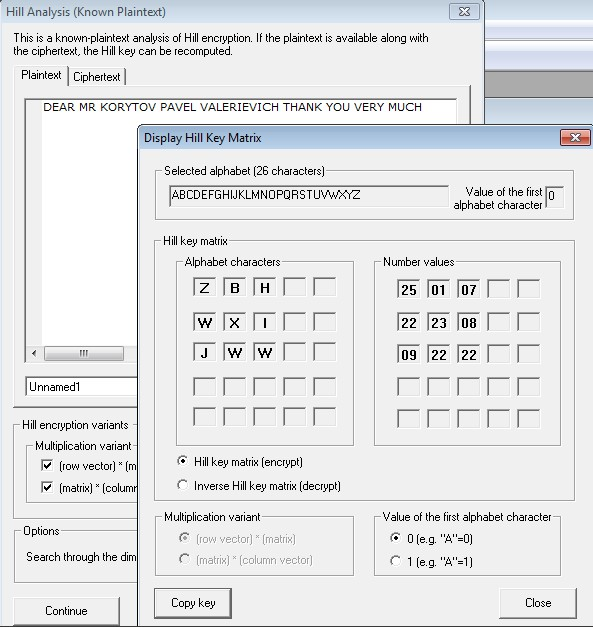
\includegraphics[width=0.8\textwidth]{./img/S004.jpg}
        \caption{Атака на шифр основе открытого текста}%
        \label{img:1:3}
    \end{figure}
    
    \item Из сообщения удалено ФИО автора. Дешифрованный ключ совпадает с исходным 
    \begin{figure}[h]
        \centering
        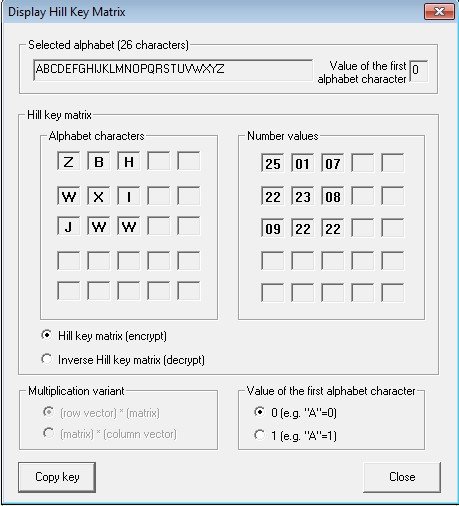
\includegraphics[width=0.8\textwidth]{./img/S005.jpg}
        \caption{Повторение атаки на основе открытого текста}%
        \label{img:1:4}
    \end{figure}
    
    \item Коллеге для дешифрования передано следующее сообщение: \texttt{LADIES AND GENTELMEN YOU HAVE WRONG UNDERSTANDING OF REASON AND THEREFORE THINK YOU EXIST FOR NO REASON THANK YOU}. Ключ --- \texttt{YJ PU}.
    Шифротекст: \texttt{XEHSCK IXN CEJDINWEJ UMG JKJQ QBEDG OFTMPKPCZVAVM KR FEWAUV KZV HTSPCXITM FDERM UMC YNAYV NUR JI TEWAUD TBSRM UMEX} 

    \item Получен следующий шифротекст: \texttt{GYHBPUMH XJZHEITSIWUJEFMLVGCQJLBENCMIIXTRRDZANIUTRRKGEXHOLEKEXQT IEFEWOTVFRY XWDETLYOOA}.

    По паре открытый текст / шифротекст --- \texttt{LADIES AND GENTELM} / \texttt{GYHBPUMH XJZHEITSI} --- восстановлен ключ --- матрица $3\times3$ \texttt{I J F L C J M Y D}. 

    Дешифрованный открытый текст: \texttt{LADIES AND GENTLEMEN WELCOME TO THE FIRST SATANIST TEMPLE ININIATION CEREMONY THANK YOU}. 

\end{enumerate}

\FloatBarrier{}
\section{Комбинированный шифр ADFGVX}
Шифрование осуществляется в два этапа. На первом этапе задается матрица, заполненная символами алфавита, а также цифрами от 0 до 9. Далее каждый символ кодируется парой символов, на пересечении которых он находится. На втором этапе производится перестановка столбцов, заданная кодовым словом.

\begin{figure}[h]
    \centering
    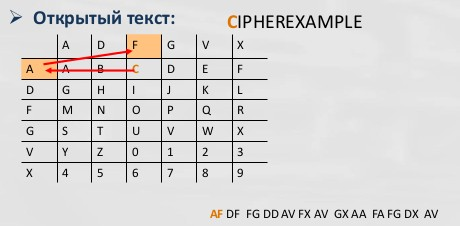
\includegraphics[width=0.95\textwidth]{./img/S001.jpg}
    \caption{Первый шаг зашифровки}%
    \label{img:2:1}
\end{figure}

\begin{figure}[h]
    \centering
    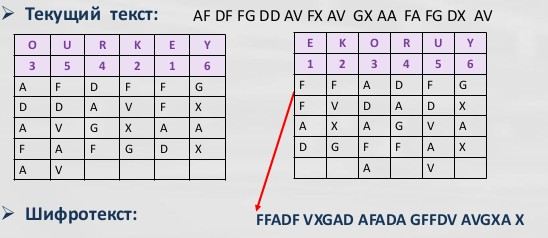
\includegraphics[width=0.95\textwidth]{./img/S002.jpg}
    \caption{Второй шаг зашифровки}%
    \label{img:2:2}
\end{figure}

\subsection{Формулировка задания}
\begin{enumerate}
    \item Найти шифр в CrypTool 1: Encrypt/Decrypt-> Symmetric (Classic).
    \item Зашифровать и расшифровать текст содержащий только фамилию (транслитерация латиницей) вручную и с помощью шифра c выбранным ключом. Убедиться в совпадении результатов.
    \item Выбрать абзац (примерно 600 символов) из файла English.txt (папка CrypTool / reference) и зашифровать его.
    \item Выполнить атаку на шифротекст, используя приложение из Analysis-> Symmetric Encryption (classic)-> Cipher Text Only.
    \item Повторить шифрование и атаку для тестов примерно в 300 и в 150 символов.
    \item Изучите ручное расшифрование для текстов менее 300 символов.
    \item Зашифруйте текст из 200 символов, сохраните ключ, и передайте соседу для расшифровки.
    \item Самостоятельно изучите атаку по словарю, реализованную в CrypTool 2, опираясь на Help и ссылки на статьи.
\end{enumerate}

\subsection{Ход работы}
\begin{enumerate}
    \item Найден шифр в CrypTool 1. Для использования шифра пришлось делать размер окна VirtualBox выше, чем размер экрана. Параметры шифра на рисунке~\ref{img:2:3}
    \begin{figure}[h]
        \centering
        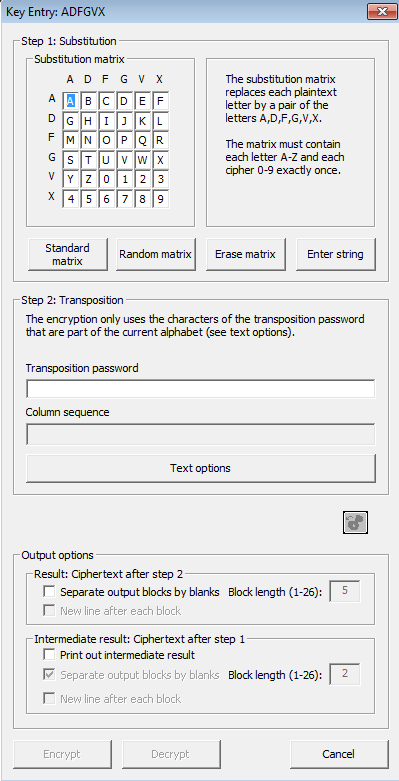
\includegraphics[width=0.7\textwidth]{./img/ADV.png}
        \caption{Параметры шифра ADFGVX}%
        \label{img:2:3}
    \end{figure}
    
    \item Фамилия автора --- \texttt{KORYTOV}, выбранный ключ: \texttt{PAVEL} 
    \begin{table}[h]
    \centering
    \begin{tabular}{@{}l|llllll@{}} % chktex 44
     & \textbf{A} & \textbf{D} & \textbf{V} & \textbf{G} & \textbf{F} & \textbf{X} \\ \midrule
    \textbf{A} & A & B & C & D & E & F \\
    \textbf{D} & G & H & I & J & K & L \\
    \textbf{V} & M & N & O & P & Q & R \\
    \textbf{G} & S & T & U & V & W & X \\
    \textbf{F} & Y & Z & 0 & 1 & 2 & 3 \\
    \textbf{X} & 4 & 5 & 6 & 7 & 8 & 9
    \end{tabular}
    \end{table}

    Результаты первого шага зашифровки: \texttt{DF VV VX FA GD VV GG}

    \begin{table}[h]
    \centering
    \begin{tabular}{@{}lllll@{}}
    \textbf{P} & \textbf{A} & \textbf{V} & \textbf{E} & \textbf{L} \\
    \textit{4} & \textit{1} & \textit{5} & \textit{2} & \textit{3} \\ \midrule
    D & F & V & V & V \\
    X & F & A & G & D \\
    V & V & G & G & 
    \end{tabular}%
    \hspace{1cm}
    \begin{tabular}{@{}lllll@{}}
    \textbf{A} & \textbf{E} & \textbf{L} & \textbf{P} & \textbf{V} \\
    \textit{1} & \textit{2} & \textit{3} & \textit{4} & \textit{5} \\ \midrule
    F & V & V & D & V \\
    F & G & D & X & A \\
    V & G &  & V & G
    \end{tabular}
    \end{table}

    Шифротекст: \texttt{FFVVG GVDDX VVAG}.
    
    Поскольку длина ключа --- 5, а длина шифротекста --- 14, в столбце с буквой, обратной последней букве ключа (\texttt{V}) будет на один символ меньше.
    \begin{table}[h]
    \centering
    \begin{tabular}{lllll}
    \toprule
    \textbf{P} & \textbf{A} & \textbf{V} & \textbf{E} & \textbf{L} \\
    \textbf{4} & \textbf{1} & \textbf{5} & \textbf{2} & \textbf{3} \\
    \textit{1} & \textit{2} & \textit{3} & \textit{4} & \textit{5} \\ \midrule
    \textbf{1} & \textbf{2} & \textbf{3} & \textbf{4} & \textbf{5} \\
    \textit{2} & \textit{4} & \textit{5} & \textit{1} & \textit{3} \\
    \textit{E} & \textit{P} & \textit{V} & \textit{A} & \textit{L} \\
    \bottomrule
    \end{tabular}%
    \hspace{1cm}
    \begin{tabular}{@{}lllll@{}}
    \textbf{E} & \textbf{P} & \textbf{V} & \textbf{A} & \textbf{L} \\
    \textit{2} & \textit{4} & \textit{5} & \textit{1} & \textit{3} \\ \midrule
    F & V & V & D & V \\
    F & G & D & X & A \\
    V & G &  & V & G
    \end{tabular}%
    \hspace{1cm}
    \begin{tabular}{@{}lllll@{}}
    \textbf{A} & \textbf{E} & \textbf{L} & \textbf{P} & \textbf{V} \\
    \textit{1} & \textit{2} & \textit{3} & \textit{4} & \textit{5} \\ \midrule
    D & F & V & V & V \\
    X & F & A & G & D \\
    V & V & G & G & 
    \end{tabular}
    \end{table}
    
    Результат первого шага расшифровки: \texttt{DF VV VX FA GD VV GG}

    Второй шаг дает исходный текст: \texttt{KORYTOV}
    
    \FloatBarrier{}
    \item Выбран абзац из Agenda 21 длиной в 600 символов и зашифрован. Результат на

    \begin{figure}[h]
        \centering
        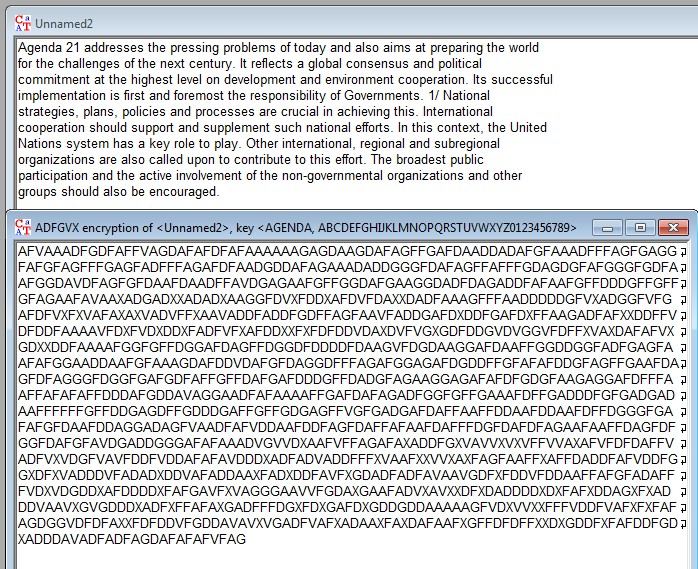
\includegraphics[width=0.8\textwidth]{./img/S006.jpg}
        \caption{Зашифровка абзаца Agenda 21}%
        \label{img:2:4}
    \end{figure}
    
\item Выполнена атака на шифротекст. Атака выполнена успешно; однако, для получения результата пришлось возвращать матрицу подстановки в стандартный вид. Результаты на рисунке~\ref{img:2:5}

    \begin{figure}[h]
        \centering
        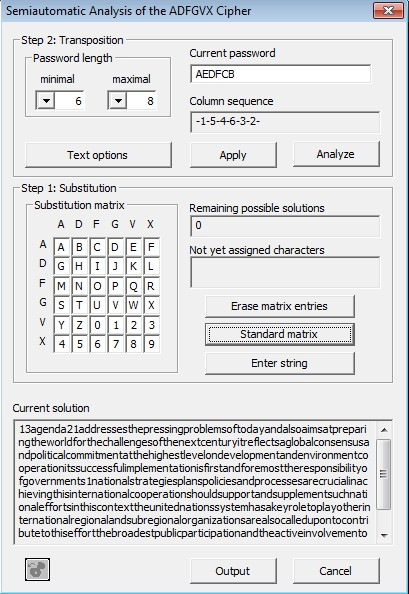
\includegraphics[width=0.6\textwidth]{./img/S007.jpg}
        \caption{Атака на шифр ADFGVX}%
        \label{img:2:5}
    \end{figure}

    \item Текст длиной в 300 символов дешифрован успешно, но количество итераций дешифровки составило 9. Для текста длиной в 150 символов число итераций приблизилось к 100.

    \item Ручное дешифрование для текстов менее 300 символов --- трудоемкая задача, особенно без вычислительного оборудования. Жорж Пенвен, взломавший шифр в 1918 году, использовал для дешифрования сообщения со стандартным началом; по повторяющимся фрагментам шифротекста определялась вероятная длина ключа.
    
    Кроме того, можно определить, какие буквы составляют столбцы, а какие --- строки, т.к. между этапами зашифровки они чередуются. Объединение четных и нечетных пар и их частотный анализ позволяли определить, являются ли они результатом замены символов открытого текста.
    
    Таким образом, требуется объемный статистический анализ, который сложно провести вручную; для недостаточного объема текста это практически невозможно.

    \item Ключом ``HUMAN'' зашифрована следующая цитата Чарльза Дарвина:
    ``When I view all beings not as special creations, but as the lineal descendants of some few beings which lived long before the first bed of the Cambrian system was deposited, they seem to me to become ennobled''

    Результат шифрования: ``DDFAX DAFAF FDXGF ADGVF AAFAD FAAVA DGFDG DDAFG VFDAX AAFAV DGAFA ADVVG AFVFV FXGVG VDDFA GAAFA VDDGA DXAXG VADAF AVDAD FDVFA AXDXG DFDAA DDGVA GFFAD GVFVA FADAV DDDVD VDDAA AAFAF AGAAF AGADF AGAAD FADDG GFDFV AFGVA DADAA GAGVG DGVAA FDAFA DDGAF AAAFG FGGDX ADFDA DDDDV AGGFF VGVDV AXAXD VFDAX AGGVF XFAAV AGDVD AADAF AAFFA VFGGX ADFDG VAFAF GFGDD VAAFA GXFXA FGDDF AFAXA DDAAF DFAFG AFAAF GGAAF FGDFV FDA''

    Сообщение передано коллеге для расшифровки.

    \item Дешифрование полученного текста
        
        От коллеги получен шифротекст: ``\texttt{FFGXX DFXDD DVDXA FFGFF DGDFV XFADD AAADX DDDAD DDFDD FVDXA VAXGX FXADF AFXGF VAGFF AVGGX DFFAF AXVFD FAFAG FDAAG AGFFD FADFD FFDGD AADFA GAGFD FFFFF DFAGD ADFAA FDFFD DGDAG FDAAA GADFG AAGFD AGGFF DADGF ADDGG AAAGF FAAFF AFGFD DGDDF GFFFA GAGAF AAFGA FDDDG AAFGA DAGAA GDDDG AAFAA AFGFA FAGAF FAADD FAVDV FFVFG VVDXF VADDV AAFFA DFXXA FAXXA VDAFV AFDVX FXVDV VXAAX ADFVV FDDFG VXAVV AAGVF VDVFX VXFXD A}''

    С помощью атаки по словарю CrypTool2 сообщение восстановлено.

    \texttt{IWONDERIFITWOULDBEBETTERTOREMAINONDEIMOSHOPINGITWILLCRASHONMARSFASTERTHANONEMANONTHEORBITLIKETHEREARESMALLPARTICLESWHICHSHOULDDECREASEDEIMOSSPEEDOVERTHECOURSEOFMILLENIA}.

    Расставлены пробелы:

    \texttt{I WONDER IF IT WOULD BE BETTER TO REMAIN ON DEIMOS HOPING IT WILL CRASH ON MARS FASTER THAN ONE MAN ON THE ORBIT LIKE THERE ARE SMALL PARTICLES WHICH SHOULD DECREASE DEMOS SPEED OVER THE COURSE OF MILLENIA} 

    Атака заняла продолжительное время; потребовался подбор длины ключа. Было отвергнуто несколько вариантов, которые расшифровывали текст бессмысслицу.

    Предположительно, текст описывает возможности схода со стабильной орбиты Марса без использования реактивной тяги.

\end{enumerate}

\FloatBarrier{}
\section{Шифр Плейфера (Playfair)}

\subsection{Описание шифра}
Исходный текст разбивается на блоки --- биграммы по 2 символа. Ключом является матрица $5\times$5.
Процесс шифрования подчиняется следующим правилам:
\begin{enumerate}
    \item Если два символа совпадают или остался один символ, то к первому символу добавляется X и шифруется уже эта пара.
    \item Если символы находятся в одной строке, то они замещаются на расположенные в ближайших от них справа символы.
    \item Если символы в одном столбце, то они замещаются на расположенные ниже в ближайших от них клетках
    \item Если символы находятся в разных углах образуемого ими прямоугольника, то они заменяются на символы, стоящие в противоположных углах этого прямоугольника, в тех же строках\\
\end{enumerate}

Расшифровка сообщения происходит инверсией данных правил

\subsection{Формулировка задания}
\begin{enumerate}
    \item Найти шифр в CrypTool 1: Encrypt/Decrypt-> Symmetric (Classic).
    \item Зашифровать и расшифровать текст содержащий только фамилию (транслитерация латиницей) вручную и с помощью шифра c выбранной ключевой матрицей. Убедиться в совпадении результатов.
    \item Зашифровать текст с произвольным сообщением в формате ``DEAR ALL THANK YOU FOR ПРОИЗВОЛЬНЫЙ ТЕКСТ'', используя выбранную шифрующую матрицу.
    \item Выполнить атаку на основе знания части открытого текста, используя приложение из Analysis-> Symmetric Encryption (classic)->Manual Analysis. В качестве известного фрагмента текста использовать `DEAR ALL THANK YOU FOR'':
    \begin{enumerate}  
        \item Познакомьтесь с методикой проведения атаки в разделе Work through the examples из Help
        \item Познакомьтесь со спецификацией приложения для проведения атаки в разделе Analysis-> Symmetric Encryption (classic)->Manual Analysis->Playfair
    \end{enumerate}
    \item Передайте произвольную шифровку соседу для расшифрования
при условии, что форма обращения, используемая в сообщении, известна.
Размер использованной матрицы (ключа) держать в секрете.
\end{enumerate}

\subsection{Ход работы}
\begin{enumerate}
    \item Найден шифр в Cryptool 1. Параметры шифра на рисунке~\ref{img:3:1}
    \begin{figure}[h]
        \centering
        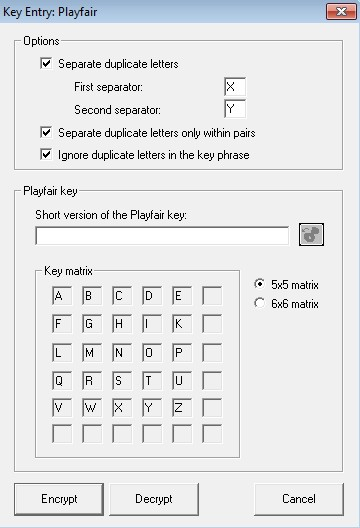
\includegraphics[width=0.7\textwidth]{./img/S008.jpg}
        \caption{Параметры шифра Playfair}%
        \label{img:3:1}
    \end{figure}
    
    \item Для ручного зашифрования выбрана следующая матрица-ключ:
    \begin{table}[h]
    \centering
    \begin{tabular}{@{}lllll@{}}
    \toprule
    R & E & M & B & W \\
    H & N & T & S & A \\
    L & I & C & D & F \\
    G & K & O & P & Q \\
    U & V & X & Y & X \\
    \bottomrule
    \end{tabular}
    \end{table}
    
    Зашифрование: \texttt{KORYTOV} $\Rightarrow$ \texttt{KO RY TO V} $\Rightarrow$ \texttt{KO RY TO VX} $\Rightarrow$ \texttt{OP BU CX XY}

    Расшифрование: \texttt{OP BU CX XY} $\Rightarrow$ \texttt{KO RY TO VX} $\Rightarrow$ \texttt{KORYTOV}
    
    \FloatBarrier{}
    \item Зашифрован следующий текст: \texttt{DEAR ALL THANK YOU FOR NOT BEING HERE AND IF YOU ARE HERE PLEASE LEAVE} с ключом \texttt{LEAVEMEBEHIND}. Результаты на рисунке~\ref{img:3:2}

    \begin{figure}[h]
        \centering
        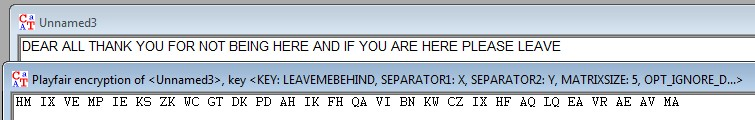
\includegraphics[width=\textwidth]{./img/S009.jpg}
        \caption{Результаты шифрования}%
        \label{img:3:2}
    \end{figure}
    
    \item Проведена атака на основе знания части открытого текста \texttt{DEAR ALL THANK YOU FOR}. На основе этой части сначала восстановлено слово \texttt{BEING}, затем --- на основе расширенного открытого текста --- проведена окончательная дешифровка. Результаты на рисунке~\ref{img:3:3}
    \begin{figure}[h]
        \centering
        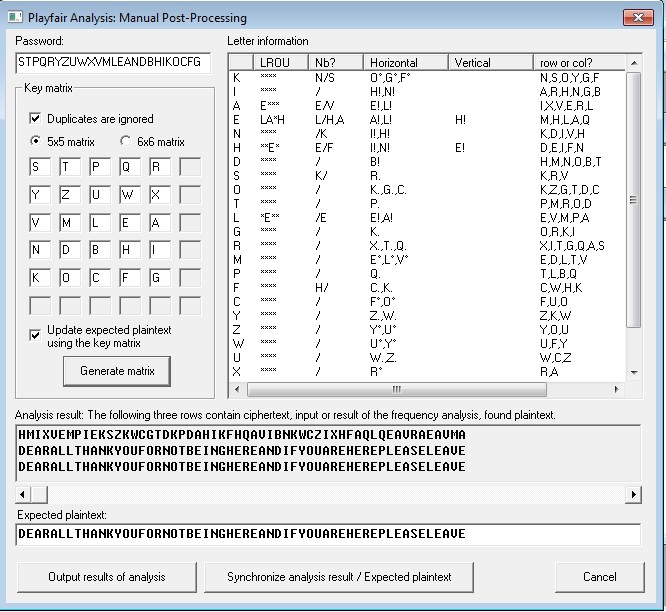
\includegraphics[width=0.8\textwidth]{./img/S010.jpg}
        \caption{Результаты атаки на шифр Плейфера}%
        \label{img:3:3}
    \end{figure}
    
    \item Коллеге зашифрована следующая цитата Ленина ключом \texttt{STATEANDREVOLUTION}: ``In capitalist society, under the conditions most favorable to its development, we have more or less complete democracy in the democratic republic. But this democracy is always restricted by the narrow framework of capitalist exploitation and consequently always remains, in reality, a democracy for the minority, only for the possessing classes, only for the rich. Freedom in capitalist society always remains about the same as it was in the ancient Greek republics: freedom for the slave owners''.

    Результат: \texttt{FT BE HF AE RF TA ED FB NA QC SL TO RW OM LE RU RH LE EG DE NI VB LV VK ON ER HR DU AO NO LM YO SA YT KT OA YC OT LV ON AQ EU CY ZF NA SO OY CM VT ME FT RW SO OY CM VT RH IO NM IC RF FC IS RW UT OS YC IO EB WC TE RZ EX TD NT RI BF AN VU WE MT SE VW VL ZI VT YO YR VH LC BE HF AE RF TA AY ZF RC AE RH LE ES OU LE TN SG NS NR XE RZ EX TD OY TB ST FT OT NV HR XE OS YC IO EB ZC LV RW OY FT LV HR EC LF ZC LV RW NM DE TN AQ TU SP FO ET TN ED LF ZC LV RW TO BF PI OT SO CY FT BE HF AE RF TA ED FB NA XE RZ EX TD OY TB ST VK DC AW RW NT EK NE TU RT ET FT RW NE EF CT SA HD AY AM OT GF FV BF NU OT SO CY CL IR MT ND VB OC ZT TO AQ}.

    Коллеге переданы следующие слова сначала: \texttt{INCAPITALISTSOCIETYUNDERTHE} 

    \item Получен шифротекст: \texttt{SK CS ON AT PU OA NS UR OK OM AQ SU NO PN PY MO GI BH NR CR SK IA KI CA PC AV EI SK BA MO BA NR CB YI ON IQ HY NA RC SC YE RK HM IP QE OM HC SK CU AD UW VD SC SF RS NR ZQ SH OM AN AT HI IU HI KL NU SE MK CS SH DI BS BU QO CA ZC UO MR SV SK CE HY QN AP SC WQ IA UC CK IH AB CZ ID NO BV ED RH TQ HE AL NE LC MK EY RS EY QC IP YO HN TL SH ZH US QZ SK CU OD MO AN LC MR SK CE HY LC AT SC RH SK HA UF MK IA NR LV HY YH WQ IA UC CK IH SE TL NS ER PL FA BF KS SH VE RC LC RS SV EN MV ID IH TQ HE AL EY SE TL RE TL SH SR LC OZ MO FG MO TQ HE ON RK LO CR IU SU PH UF HK PZ CL SY OU IL TL SH VH IY IS UW IH NR UY MH DM HY LE YI DU HK LC MK TL VS CS SH HI HU AT DR HY DE IS FV RS PV EY ME NR FR AC FG MO NA MO HE QM DM HY LE YI EP UH MO ON BM RB MK CR PN CA BA AY RP LD IA YE RK EP CR KQ SH YS MO QK SR LD EP NS BY LN BA IS ZE PR YH ON MK CS DE TQ AI YI CZ IH YE AR CL HY SU NO AB RN RK HM QV VD ET OU IL QA CA DO MA SE RD MK CA UF HK OM MA PN AN AC IW IA SK EL YO TE MA EU AC FV CL KS SH AN RC QP HY AY SC BG AI NH CR KQ SH TL UD PW SE SR MZ CR PN AN AZ DP BY UE SI YH KZ UR AT NR HL BE YH KZ UR AT CL SO DL LD RD HI RK LE CZ SH WF RC EN RK AN IC FR RC NR YO AL EY SK IA MA NR TE UF VL EC AM AI DP BY UE SI SK NR SK US SE SR MZ NR HL LC QV PL UF HK IA SK NR SK BH OE PT NR LD EC ID NR QY}

        Известное обращение: \texttt{THETRANSFORMATIONFROMSPEAR}. После восстановления некоторых слов восстановлен исходный текст (пробелы расставлены): 

        \texttt{THE TRANSFORMATION FROM SPEAR TO SWORD BEGAN IN THE 3RD CENTURY BC THE MORE MANEUVERABLE SAMNITES AND GAULS BROKE THEIR HOPLITE PHALANX THE ROMANS DECIDED TO CHANGE THEIR EQUIPMENT NOW ONLY THE BEST MOST EXPERIENCED MEN TRIARII HAD SPEARS ACTING AS A LAST BULWAK AS THEY KEPT THEIR FORMATION THE BEST INSTEAD THE YOUNGER AND LESS EXPERIENCED HASTATI ALTHOUGH THEY INITIALLY CARRIED SPEARS AS HASTA IS THE LATIN WORD FOR SPEAR AND PRINCIPES FOUGHT WITH SWORDS THEY DEVELOPED A NEW AGGRESSIVE FIGHTING STYLE THE DEFENSIVE SHIELD WALL WAS ABANDONED FOR A MORE AGGRESSIVE USE FOR RAMMING INTO ENEMY SOLDIERS AND USING THE SHORT GLADIUS AT EXTREMELY CLOSE RANGE THIS PREVENTED SAMNITE SPEARMEN AND GALLIC SWORDSMEN FROM HAVING ENOUGH ROOM TO MANEUVER THIS WAS COMBINED WITH THE MANIPLE SYSTEM BREAKING THE STIFF PHALANX INTO MANY FLEXIBLE SECTIONS AND SUBSECTIONS IT PAID DIVIDENDS IN THE PUNIC AND MACEDONIAN WARS AS THE ROMANS COULD BE MORE FLEXIBLE THAN THE PHALANX AND STILL TOUGHER THAN THE GAULS AND IBERIANS} 

        Текст описывает, как гастаты вытеснили триариев с передних рядов боевых легионов Римской Республики.
\end{enumerate}


\newpage
\section*{Выводы}
\begin{table}[h]
    \begin{tabularx}{\textwidth}{@{}XXXX@{}}
    \toprule
    \textbf{Название шифра} & \textbf{Тип шифра} & \textbf{Ключ} \\ \midrule
    \textit{Hill} & Замена & Шифрующая матрица \\
    \textit{ADFGVX} & Комбинированный & Матрица, ключевое слово \\
    \textit{Playfair} & Замена & Матрица \\ \bottomrule
    \end{tabularx}
\end{table}

\begin{table}[h]
    \begin{tabularx}{\textwidth}{@{}XX@{}}
        \toprule
        \textbf{Название шифра} & \textbf{Сложность brute force} \\ \midrule
        \textit{Hill} & $ 26^{n^2} $, где $n$ --- размер матрицы. Если неизвестен, то $ n \le \log_{2}(l) $, где $l$ --- длина сообщения \\
        \textit{ADFGVX} & $ \Factorial{36} \times \Factorial{n} $, где $n$ --- длина ключа. Если неизвестно --- длина сообщения. \\
        \textit{Playfair} & $\Factorial{m}$, где $m$ --- размер матрицы.  \\
        \bottomrule
    \end{tabularx}
\end{table}

Шифр Hill --- сложный в использовании из-за обращения матриц. Эту операцию непросто провести вручную (особенно для больших матриц), на вычислительном оборудовании это тоже неэффективно. В то же время, для взлома шифра достаточно решить систему линейных уравнений, зная небольшое количество исходного текста, что является тривиальной задачей.

Шифр ADFGVX --- самый криптоустойчивый из рассмотренных. Его ручной взлом затрудняет его комбинированная структура; однако это возможно. На современном вычислительном оборудовании взлом осуществить легко. Увеличение количества шифротекста облегчает взлом, что свидетельствует о плохой масштабируемости решения.

Шифр Playfair --- самый простой из рассмотренных. Для его взлома достаточно 15--25 символов с начала текста.

\end{document}
